\documentclass[11pt]{article}
\renewcommand{\baselinestretch}{1.05}
\usepackage[spanish]{babel}
\usepackage[utf8]{inputenc}
\usepackage{lipsum}

\usepackage{amsmath,amsthm,verbatim,amssymb,amsfonts,amscd}
\usepackage{graphicx, wrapfig}
\usepackage{float}
\usepackage{caption, subcaption}
\usepackage{tkz-fct}
\usetikzlibrary{babel}
\usepackage{pgfplots}
\usepackage{enumitem}
\usepackage{multicol, vwcol}
\usepackage{listingsutf8}
\usepackage{color}
\usepackage{hyperref}
\usepackage{booktabs}
\usepackage{ marvosym }
\usepackage[sorting=none]{biblatex}
\bibliography{bibliography.bib}
\definecolor{lightgray}{gray}{0.95}

\hypersetup{
    bookmarks=true,         % show bookmarks bar?
    unicode=false,          % non-Latin characters in Acrobat’s bookmarks
    pdftoolbar=true,        % show Acrobat’s toolbar?
    pdfmenubar=true,        % show Acrobat’s menu?
    pdffitwindow=false,     % window fit to page when opened
    pdfstartview={FitW},    % fits the width of the page to the window
    pdftitle={Ingeniería, empresa y sociedad - Entrega 1},    % title
    pdfauthor={Francisco Luque, María del Mar Ruiz},     % author
    pdfsubject={Ingeniería, Empresa y Sociedad},   % subject of the document
    pdfnewwindow=true,      % links in new PDF window
    colorlinks=true,        % false: boxed links; true: colored links
    linkcolor=red,          % color of internal links (change box color with linkbordercolor)
    citecolor=cyan,         % color of links to bibliography
    filecolor=magenta,      % color of file links
    urlcolor=blue           % color of external links
}

\setlength{\parindent}{0pt}
\topmargin0.0cm
\headheight0.0cm
\headsep0.0cm
\oddsidemargin0.0cm
\textheight23.0cm
\textwidth16.5cm
\footskip1.0cm
\theoremstyle{plain}

\newtheorem{theorem}{Teorema}
\newtheorem{corollary}{Corolario}
\newtheorem{lemma}{Lema}
\newtheorem{proposition}{Proposición}
\theoremstyle{definition}
\newtheorem{definition}{Definición}
\newtheorem{example}{Ejemplo}

\newcommand{\N}{\mathbb{N}}
\newcommand{\Z}{\mathbb{Z}}
\newcommand{\Q}{\mathbb{Q}}
\newcommand{\C}{\mathbb{C}}
\newcommand{\R}{\mathbb{R}}

\begin{document}

\title{Ingeniería, Empresa y Sociedad \\
  DGIIM \\
  \large Estudio demográfico del tejido empresarial en España: La
  importancia de las grandes empresas}
\author{Francisco Luque Sánchez\\
  María del Mar Ruiz Martín}
\maketitle

En esta práctica realizaremos un pequeño análisis sobre la situación
de las grandes empresas en España. Sustentaremos este estudio en cinco
gráficos, que nos servirán para sacar algunas conclusiones al respecto.

\section{Gráfica 1: Evolución del número de grandes empresas en
  España}

La primera gráfica que mostraremos resumirá la información sobre la
distribución de las grandes empresas a lo largo de los últimos años.
La gráfica en cuestión es la siguiente:

\begin{figure}[H]
  \centering
  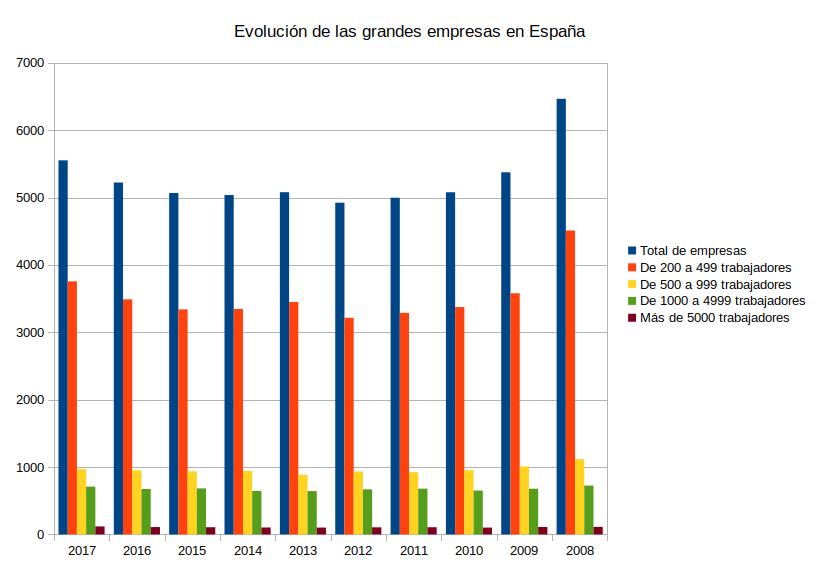
\includegraphics[width=.8\textwidth]{graficos/barras_evolucion_anual}
  \caption{Evolución del tamaño de las empresas en España}
\end{figure}


Pasamos a mostrar la tabla que recoge los datos anteriores con el fin
de facilitar el análisis de la situación:

\begin{table}[H]
\centering
\begin{tabular}{|l|l|l|l|l|l|l|l|l|l|l|}
\hline
  & 2017  & 2016  & 2015  & 2014  & 2013  & 2012  & 2011  & 2010 &  2009 &  2008\\
\hline
Total de empresas & 5552  & 5223  & 5067  & 5037  & 5079  & 4923  & 4997  & 5078 &  5375 &  6465\\
De 200 a 499 trabajadores & 3756  & 3489  & 3340  & 3346  & 3450  & 3214  & 3288  & 3374 &  3578 &  4511\\
De 500 a 999 trabajadores & 969 & 951 & 937 & 942 & 885 & 935 & 923 & 952 & 1008 &  1117\\
De 1000 a 4999 trabajadores & 709 & 674 & 683 & 646 & 643 & 669 & 679 & 651 & 678 & 725\\
Más de 5000 trabajadores  & 118 & 109 & 107 & 103 & 101 & 105 & 107 & 101 & 111 & 112\\
\hline

\end{tabular}
\caption{Evolución del tamaño de las empresas en España}
\end{table}

Lo más relevante que se puede comentar al principio es la disminución
total del número de grandes empresas desde 2008. Probablemente debido
a la crisis, entre el año 2008 y el año 2009 se produce una
disminución en el número de grandes empresas de más de 1000. Esta
disminución se mantiene, aunque de forma menos pronunciada, hasta
2012, cuando se pasan de unas 6500 empresas (2008) a menos de 5000
(2012). A partir de ese año empieza a verse una ligera recuperación en
el número total de empresas, pero
no se han conseguido alcanzar los niveles de hace 10 años, contando tan 
solo con un 85\% de las empresas presentes en 2008.\\

Otro comportamiento a tener en cuenta es que esta disminución ha
afectado principalmente a las empresas de menor tamaño dentro de las
grandes empresas. Mientras que las empresas de más de 5000
trabajadores apenas se han visto afectadas (de hecho, en el periodo de
9 años que se contempla, ha aumentado el número de éstas en 6), así
como las que tienen enter 500 y 5000 trabajadores, las que tienen
entre 250 y 499 sí que se han visto fuertemente afectadas, disminuyendo
en este periodo en casi un 17\%. Esto nos
lleva a concluir que la crisis económica en la que se ha visto sumido
el país ha afectado con mayor fuerza a empresas de pequeño tamaño,
mientras que las más grandes han salido mejor paradas.

\section{Gráfica 2: Distribución de las grandes empresas por comunidad
  autónoma}

La siguiente gráfica que comentaremos es un diagrama de sectores que
nos indica el número de empresas que hay en cada comunidad autónoma.
De nuevo mostraremos la gráfica seguida de la tabla que recoge los
datos.

\begin{figure}[H]
  \centering
  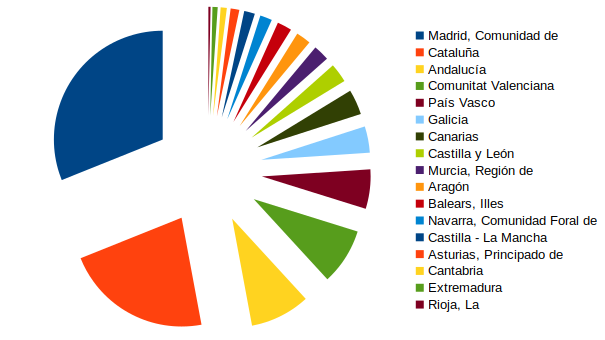
\includegraphics[width=\textwidth]{graficos/sectores_comunidades}
  \caption{Distribución de las grandes empresas en el territorio
    español}
\end{figure}

\begin{table}[H]
  \centering
  \begin{tabular}{|l|l|}
    \hline
    Comunidad Autónoma & Total Empresas \\
    \hline
    Madrid, Comunidad de  & 1723\\
    Cataluña  & 1212\\
    Andalucía & 493\\
    Comunitat Valenciana  & 464\\
    País Vasco  & 325\\
    Galicia & 217\\
    Canarias  & 208\\
    Castilla y León & 158\\
    Murcia, Región de & 131\\
    Aragón  & 122\\
    Balears, Illes  & 120\\
    Navarra, Comunidad Foral de & 99\\
    Castilla - La Mancha  & 89\\
    Asturias, Principado de & 72\\
    Cantabria & 51\\
    Extremadura & 43\\
    Rioja, La & 18\\
    \hline

  \end{tabular}
  \caption{Distribución de las grandes empresas por comunidad
    autónoma}
\end{table}

Como era esperable, más de un tercio de las grandes empresas de
nuestro país tienen su sede en Madrid. Además, entre Madrid y
Barcelona aglutinan más de la mitad de las mismas. Después, nos
aparece Andalucía (comunidad más grande de España), la Comunidad
Valenciana y el País Vasco. Coinciden las comunidades autónomas más
pobladas con las que más empresas poseen.\\

En el otro extremo tenemos a La Rioja, Extremadura y Cantabria,
contanto las tres con tan solo un 2\% del total. Coincide que estas
tres han sido históricamente las comunidades autónomas menos pobladas
y con menos riqueza del país.

\section{Gráfica 3: Filiales de empresas españolas en el exterior}

Ahora vamos a comentar la información referente a empresas filiales de
empresas españolas en el resto del mundo. Separaremos dicha
información en los siguientes cinco grupos:

\begin{itemize}
\item Zona Euro
\item Resto de la Unión Europea
\item Resto de Europa
\item América
\item Resto del mundo
\end{itemize}

Mostramos en la siguiente tabla los datos recogidos:

\begin{table}[H]
  \centering
  \begin{tabular}{|c|c|c|c|}
    \hline
    &  Número de filiales &  Personas  ocupadas & Volumen de negocio \\
    \hline
    Zona Euro & 84  & 86.665  & 13.104.888 \\
    Resto Unión Europea & 58  & 75.778  & 27.801.265 \\
    Resto Europa  & 28  & 22.759  & 2.309.599 \\
    América & 223 & 291.904 & 65.055.377 \\
    Resto del Mundo & 76  & 55.640  & 6.226.124 \\
    \hline
  \end{tabular}
  \caption{Distribución de filiales de las empresas españolas en el extranjero}
\end{table}

La gráfica en cuestión es la siguiente:

\begin{figure}[H]
  \centering
  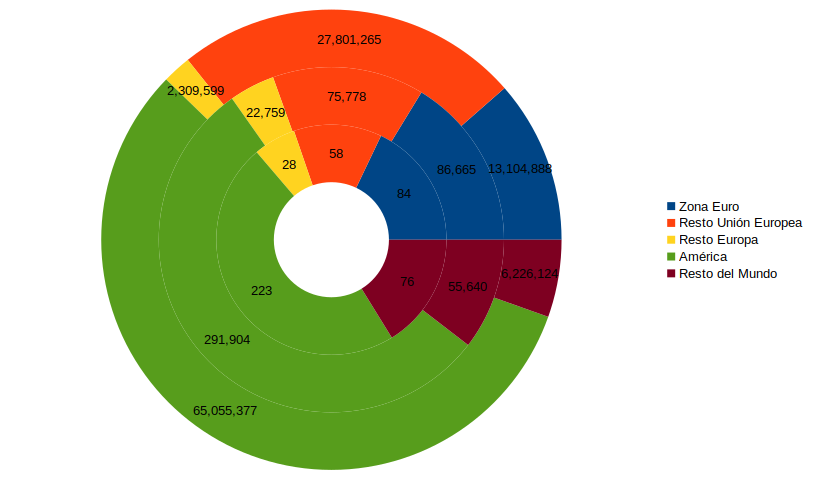
\includegraphics[width=\textwidth]{graficos/sectores_filiales}
  \caption{Distribución de filiales de las empresas españolas en el
    extranjero}
\end{figure}

En la gráfica anterior recogemos, de dentro hacia fuera, información
sobre el número de filiales en cada zona mencionada, el número de
personas ocupadas en dichas empresas, y el volumen de negocio que
generan las mismas. Podemos observar que, si ponemos atención a la
proporción volumen de negocio entre número de empresas, las que tienen
un valor más alto son el resto de la Unión Europea (esto engloba
principalmente a Suiza, al Reino Unido, y a los países escandinavos) y
América. Estas son las zonas más ricas del planeta, por lo que tiene
sentido que se produzca este fenómeno.

\section{Gráfica 4: Productividad en el sector servicios}

En esta sección se muestra la productividad media de los trabajadores
dedicados al sector servicios, separados por subsectores.  De esta
forma queremos estudiar los puestos de trabajo con mayor rentabilidad
dentro de este sector. Con estos datos obtenemos la siguiente gráfica
y tabla:

\begin{figure}[H]
  \centering
  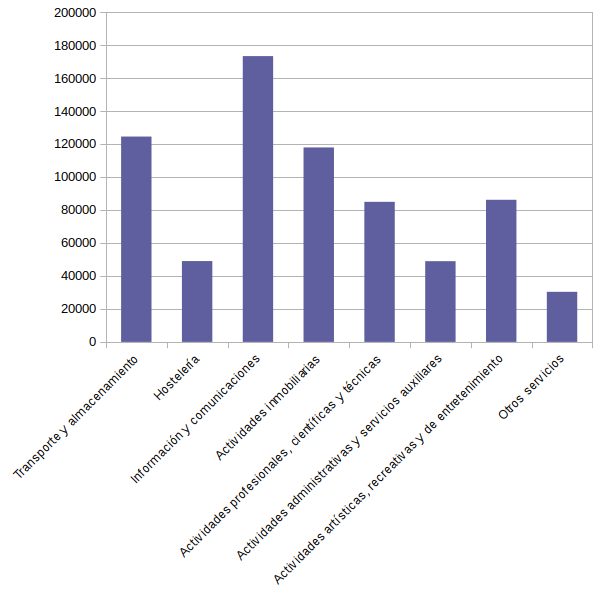
\includegraphics[width=\textwidth]{graficos/barras_productividad_servicios}
  \caption{Productividad de los trabajadores dentro del sector
    servicios}
\end{figure}

\begin{table}[H]
  \centering
  \begin{tabular}{|c|c|c|c|}
    \hline
    &\EUR por persona & Millones de \EUR & Miles de personas\\
    \hline
    Transporte y almacenamiento & 124514,087870105  & 104293  & 837,6\\
    Hostelería  & 49022,6394257316  & 62146 & 1267,7\\
    Información y comunicaciones  & 173298,092392553  & 75402 & 435,1\\
    Actividades inmobiliarias & 117911,025145068  & 24384 & 206,8\\
    Actividades profesionales,  & 84943,3500051036  & 83219 & 979,7\\
    científicas y técnicas &&&\\
    Actividades administrativas   & 48967,1255548033  & 65092 & 1329,3\\
    y servicios auxiliares &&&\\
    Actividades artísticas, recreativas& 86159,793814433 & 26744 & 310,4\\
    y de entretenimiento  & & & \\
    Otros servicios & 30367,5712813466  & 8840  & 291,1\\
    \hline
  \end{tabular}
  \caption{Produtividad de los trabajadores del sector servicios}
\end{table}

En la gráfica se muestra la cantidad de dinero generada por puesto de
trabajo en el sector servicios en el año 2015. Podemos observar que,
dentro de este sector, los trabajos más rentables son los relacionados
con las comunicaciones, seguidos por los de transporte y
almacenamiento, y las actividades inmobiliarias. En el otro extremo,
tenemos la hostelería, los puestos de administración y servicios
auxiliares, y otros servicios. Podemos encontrar entre ambos extremos
una diferencia del 410\%.

\section{Gráfica 5: Productividad por sectores}

Finalmente analizaremos el reparto de trabajadores por sectores en 
España. Para ello mostraremos una tabla con los datos obtenidos en 
2015 junto con un gráfico en el que se puede observar dicho reparto.
En él podremos observar cómo se reparten los trabajadores por 
sectores, así como la productividad de los mismos. 

\begin{figure}[H]
  \centering
  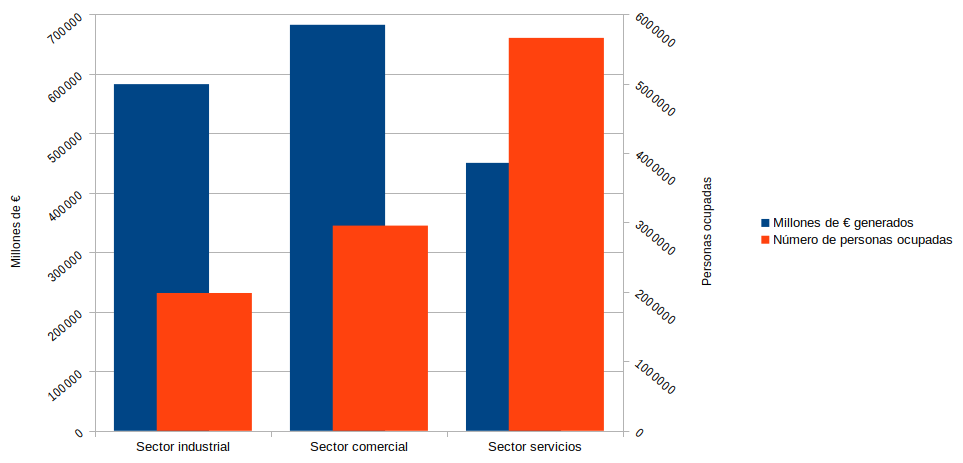
\includegraphics[width=\textwidth]{graficos/barras_sectores}
  \caption{Distribución de la actividad económica por sectores}
\end{figure}


\begin{table}[H]
  \centering
  \begin{tabular}{|c|c|c|}
    \hline
    & Millones de \EUR  generados & Número de personas ocupadas\\
    \hline
    Sector industrial & 582357 &  1984100\\
    Sector comercial &  682058 &  2955000\\
    Sector servicios &  450120 &  5657800\\

    \hline

  \end{tabular}
  \caption{Produtividad por sectores en el año 2015}
\end{table}

Podemos ver en el gráfico cómo se reparte la actividad económica por
sectores en España. Las barras azules, las cuales se interpretan con
el eje de ordenadas izquierdo, representan los millones de euros
generados durante el año 2015. Como podemos observar, el sector que
genera una mayor actividad económica es el sector comercial, con casi
700000 millones de euros anuales. Después, tenemos el sector
industrial, y finalmente el sector servicios. Por otro lado, tenemos
las barras naranjas, que representan el número de personas ocupadas en
cada sector. En este caso, el sector industrial es el que menos
puestos de trabajo genera, seguido del comercial, y finalmente el
sector servicios, que es el que emplea a un mayor número de personas.
En este gráfico se observa un comportamiento curioso. El sector
servicios, que es el que más empleo genera, es también el menos
rentable. Se ve claramente que la cantidad de dinero que genera cada
puesto de trabajo en el sector servicios es muy inferior a las otras
dos.

\end{document}
